% -----------------------------------------------
% Template for JIM
%     jim.sty -> style file
% By Eloi Batlle (eloi@iua.upf.es), changes for 
% ICMC by Bram de Jong (bdejong@iua.upf.es)
% changes for JIM 2007 by Dominique Fober (fober@grame.fr)
% changes for JIM 2009 by Olivier Tache (olivier.tache@imag.fr)
% -----------------------------------------------

\documentclass{article}
\usepackage{jim}
\usepackage{amsmath}
%\usepackage{pslatex}
\usepackage[utf8]{inputenc}
\usepackage[francais]{babel}
\usepackage[T1]{fontenc}
%\usepackage{pxfonts}
\usepackage{graphicx}
\usepackage{amssymb}
%\usepackage{multicol}

\setlength{\fboxsep}{2mm}
%\renewcommand{\submitted}{
%\begin{figure}[b]
%  \framebox[80mm]{\footnotesize{Cet article a été soumis aux JIM 2010.}}
%\end{figure}
%}

\newcommand{\emptyseg}		{\ensuremath{\oslash}}
\newcommand{\seg}[1]			{Seg(#1)}
\newcommand{\lra}				{$\leftrightarrow$}
\newcommand{\rshift}			{\hspace*{4mm}}
\newcommand{\osc}[1]			{{\small \texttt{#1}}}

\hyphenation{éten-dre com-pte gra-phi-ques adres-se ex-emple}

% Title.
% ------
\title{Partitions musicales augmentées}
\author{D. Fober, C. Daudin, S. Letz, Y. Orlarey\\
{\small \{fober,daudin,letz,orlarey\}@grame.fr}\\
Grame - Centre national de création musicale
}

%\footnote{Cet article a été soumis aux JIM 2010.}

% Single \textsc{address}
% To use with only one author or several with the same address
% ---------------
%\oneauthor
%  {Author} {School \\ Department}

% Two addresses
% --------------
%\twoauthors
%  {First author} {School \\ Department}
%  {Second author} {Company \\ Address}

% Three addresses
% --------------
%\threeauthors
%  {Auteur 1} {Grame  \\ Adresse électronique}
%  {Auteur 2} {Organisme \\ Adresse électronique}
%  {Auteur 3} {Organisme \\ Adresse électronique}

\begin{document}
%
\maketitle
%
\begin{abstract}
Une \emph{partition musicale augmentée} est une partition mettant en relation un objet musical symbolique avec différentes représentations de son interprétation. La partition musicale est à considérer au sens large, comme un objet graphique permettant de représenter un objet temporel. L'interprétation représente une instance sonore ou gestuelle particulière de la partition. Nous présenterons les fondements théoriques qui sous-tendent la \emph{partition augmentée}, ainsi qu'une application sous forme d'\emph{afficheur} mettant en oeuvre les solutions proposées.
\end{abstract}

%-------------------------------------------------------------------------
\section{Introduction}\label{sec:introduction}

La notation musicale s'inscrit dans une longue histoire et a beaucoup évolué à travers les âges. Des neumes aux notations contemporaines, notre culture est riche de toutes les voies explorées pour représenter la musique. Des formes symboliques ou prescriptives de la notation aux représentations purement graphiques \cite{brown}, la partition musicale reste en constante interaction avec le processus de création artistique.

Cependant, bien que l'on ait assisté à une explosion des représentations avec l'avènement de l'informatique musicale  \cite{dann93b,selfridge-field97,hewlett01}, la partition, destinée à l'interprète, n'a pas évolué en proportion des nouvelles formes musicales. En particulier, il y a un fossé important entre les musiques interactives et la manière statique de les représenter. L'interprête ne dispose souvent que d'une partition traditionnelle à laquelle s'ajoute une représentation électronique minimale de l'état du système, sous forme rudimentaire de compteur ou de lettres.
%Une des raisons importante de cette \emph{inertie} tient probablement au fait que la partition s'est structurée au fil des siècles autour de l'optimisation de sa lecture.


La notation musicale par ordinateur a toujours été et demeure une tâche complexe \cite{BIRD84}. En dehors du monde commercial de l'édition de partition, les systèmes les plus aboutis, 
i.e. ceux qui vont au delà de la notation traditionnelle, proposent des approches de type gravure musicale \cite{Hamel98,lilypond03}. Bien que n'ayant pas l'ambition de produire des 
partitions mises en page, l'approche proposée par ENP \cite{KUUSK06} est certainement la plus ouverte à l'extension de la notation, notamment grâce au langage Lisp sur lequel s'appuie ENP. 
Toutefois aucune de ces approches ne permettent la prise en compte d'aspects dynamiques dans la partition.

A partir du constat que le temps est une propriété commune à tous les objets musicaux, nous proposons d'étendre la partition musicale à tout objet graphique possédant des propriétés temporelles. Nous appellerons \emph{partition musicale augmentée}, l'espace permettant de représenter, composer et manipuler des objets musicaux hétérogènes, aussi bien dans le domaine graphique que temporel. La définition des propriétés graphiques et temporelles requises définit dans le même temps toute une classe de partitions musicales.

Nous allons considérer des objets arbitraires (partitions musicales, images, texte, représentation du signal, graphiques vectoriels) comme candidats possibles d'une partition augmentée en leur donnant une position et une dimension temporelles nécessaires à leur statut de partition musicale, ce qui implique également de rendre les relations temporelles visibles. 

L'organisation consistante de l'espace graphique par rapport à l'espace temporel est à la base de la notation musicale traditionnelle. Elle a toutefois été bousculée dans les cinquante dernières années \cite{boucou} et particulièrement avec les languages informatiques pour la composition musicale, en raison notamment de la nature particulière de la composition algorithmique. Cependant, la question de cette consistance reste ouverte, y compris dans les recherches récentes \cite{bresson08} aussi bien que pour satisfaire les besoins de synchronisation de différents médias \cite{baggi09b,ludo06}.

La synchronisation dans le domaine graphique de médias hétérogènes soulève des questions de non-linéarité, discontinuité, non-bijectivité. Nous avons abordé ces questions par le biais de la \emph{segmentation} et de la description de relations entre \emph{segments}. 

Enfin, la représentation de l'interprétation musicale, soit gestuelle ou sonore, est abordée avec un renversement de perspective : la représentation graphique d'un signal y est vue comme un \emph{signal graphique}, c'est à dire comme un signal composite comportant toute l'information nécessaire à son rendu graphique. Cette approche, qui abstrait le calcul de la représentation, constitue un système ouvert et dynamiquement extensible.

Nous nous attacherons tout d'abord à décrire les principes de base des \emph{mappings} ainsi que le contexte de leur utilisation dans le cadre de la partition augmentée. Nous expliquerons ensuite comment le système traite les signaux de l'interprétation pour en faire des \emph{signaux graphiques}. Enfin nous présenterons l'\emph{afficheur} de partitions augmentées en nous attachant plus particulièrement à son API de contrôle qui est une API de messages OSC\cite{wright02}.


%------------------------------------------------------------
\section{Relations temporelles et graphiques}
%------------------------------------------------------------

Nous parlerons de \emph{synchronisation temporelle dans le domaine graphique} pour faire référence à la représentation graphique des relations temporelles entre composants d'une partition. 
Notre expérience dans ce domaine \cite{chapuis07,Fober:07a} nous a conduit à aborder la question de ces relations par le biais de la \emph{segmentation} et de la description de relations entre \emph{segments}. Nous utiliserons par la suite le terme \emph{mappings} pour faire référence à ces relations.

Le rôle d'un \emph{mapping} est d'établir des correspondances entre les \emph{segments} de ressources différentes. Un \emph{segment} est une zone contiguë d'une ressource.
Ainsi que mentionné en introduction, ces ressources peuvent être de nature arbitraire (images, texte, notation musicale, signaux...). Ces mappings permettent typiquement de lier des positions graphiques, du temps musical et des positions dans des ressources audio.

Un mapping entre un enregistrement audio et une partition musicale permet par exemple d'exprimer une correspondance entre une position audio (exprimée en frames) et un temps musical 
(exprimé en subdivision de la noire). Un mapping entre une partition musicale et sa représentation graphique permet d'exprimer une correspondance entre une position exprimée en temps musical 
et une position graphique. La combinaison de ces mappings suffit alors à exprimer des relations entre toutes les ressources ayant une base temporelle.

Les sections qui suivent définissent un cadre général pour les notions de \emph{segment, segmentation} et \emph{mapping}. Ces définitions sont indépendantes de toute implémentation et de toute information spécifique aux différentes ressources. Elles sont suivies de cas concrets d'utilisation, implémentés dans le cadre de l'afficheur de partition augmentée.


%----------------------------------------------------------------
\subsection{Definitions}
%----------------------------------------------------------------

Nous allons tout d'abord introduire les notions de segments graphiques et temporels. Puis nous généraliserons ces définitions concrètes en une version abstraite et générique.


\subsubsection{Segment temporel}
%----------------------------------------------------------------

Un \emph{segment temporel} est défini comme un intervalle
 $i=[t_{0},t_{1}[$ tel que $t_{0} \leqslant t_{1}$.

Un intervalle $i=[t_{0},t_{1}[$ est dit vide quand $t_{0} = t_{1}$. Il sera noté \emptyseg.

%L'union et l'intersection de segments temporels sont tels que communément définies:
L'intersection de segments temporels est telle que communément définie: c'est le plus grand intervalle tel que 
\[ \forall i_{m},\ \forall  i_{n}, 
\ i_{m} \cap i_{n}  := \{ j \ |\ j \in i_m \ \land\ j \in i_n \}
\]


%----------------------------------------------------------------
\subsubsection{Segment graphique}
%----------------------------------------------------------------
Un \emph{segment graphique} $g$ est défini comme un rectangle donné par deux intervalles $g=(i_x,i_y)$ où $x$ est un intervalle sur l'axe des abscisses et $y$, sur l'axe des ordonnées.

Un segment graphique $g=(i_x,i_y)$ est dit vide quand $i_x = \emptyseg $ ou $i_y = \emptyseg $

L'opération d'intersection $\cap$ entre segments graphiques est définie telle que:
{\small
\[ \forall g=(i_x,i_y),\ \forall  g'=(i'_x,i'_y),\ 
g \cap g' = (i_x \cap i'_x, i_y \cap i'_y)
\]
}

%----------------------------------------------------------------
\subsection{Generalisation de la notion de segment}
\label{segments}
%----------------------------------------------------------------

Nous allons étendre les notions de segment temporel et graphique à une définition plus générale de segment à $n$ dimensions.
Un segment de dimension $n$, noté $s^n$, est défini comme une liste de $n$ intervalles $s^n=(i_1,...,i_n)$ où $i_j$ est un intervalle sur la dimension $j$.

Un segment $s^n$ de dimension $n$ est dit vide quand\\ $\exists i \in s^n\ |\ i = \emptyseg $

L'intersection de segments de dimension $n$ est définie comme la liste des intersections de leurs intervalles :
\begin{equation}
s_1^n \cap s_2^n = (i_1 \cap j_1, ... , i_n \cap j_n)
\end{equation}
où $s_1^n = (i_1, ... , i_n)$ et  $s_2^n = (j_1, ... , j_n)$


%----------------------------------------------------------------
\subsection{Segmentation d'une ressource}
\label{segmentation}
%----------------------------------------------------------------
%Une ressource \emph{segmentable} $R$ est une ressource à $n$ dimensions définie par un segment $S^n$ de dimension $n$.

Une ressource $R$ de dimension $n$ est \emph{segmentable} quand elle peut être vue comme un segment $S^n$ de dimension $n$.
La segmentation d'une ressource $R$ est l'ensemble des segments
$\seg{R}=\{ s_1^n, ... s_i^n\}$ tels que : \\
\begin{displaymath}
\begin{array}{rll}
\forall i, j \in \seg{R} & i \cap j =  \emptyseg  & $les segments sont disjoints$ \\
\forall i \in \seg{R} & i \cap S^n = i & $tous les segments sont $ \\
	& & $inclus dans la ressource$ \\
\end{array}
\end{displaymath}


%----------------------------------------------------------------
\subsection{Mapping}
\label{resmap}
%----------------------------------------------------------------

Un \emph{mapping} est une relation entre \emph{segmentations}.

Pour un mapping $M\subseteq \seg{R_{1}}\times \seg{R_{2}}$ nous définissons deux fonctions:
\begin{equation}
	M^{+}(i)=\{ i'\in \seg{R_{2}}\ |\ (i,i')\in M\}
\end{equation}
qui donne l'ensemble des segments de $R_{2}$ associés au segment
$i$ de $R_{1}$. 

et la fonction inverse:
\begin{equation}
	M^{-}(i')=\{ i \in \seg{R_{1}}\ |\ (i,i') \in M\}
\end{equation}
qui donne l'ensemble des segments de $R_{1}$ associés au segment $i'$ de $R_{2}$.

Ces fonctions sont définies sur un ensemble de segments comme l'union des mappings de chaque segment :
\begin{equation}
	M^{+}(\{i_1, ...i_n\}) = \{ M^{+}(i_1) \cup M^{+}(i_2) ...  \cup M^{+}(i_n) \}
\end{equation}
et
\begin{equation}
	M^{-}(\{i_1, ...i_n\})=\{ M^{-}(i_1) \cup M^{-}(i_2) ...  \cup M^{-}(i_n) \}
\end{equation}


%----------------------------------------------------------------
\subsection{Composition de mappings}\label{subsec:compmap}
La composition de mappings se fait de manière naturelle.
Pour les mappings $M_{1}\subseteq \seg{R_{1}}\times \seg{R_{2}}$ \\
et $M_{2}\subseteq \seg{R_{2}}\times \seg{R_{3}}$ :
\begin{equation}
(M_{1} \circ M_{2})^{+}(i) = M_2^{+}(M_1^{+}(i))
\end{equation}
De manière similaire :
\begin{equation}
(M_{1} \circ M_{2})^{-}(i') = M_1^{-}(M_2^{-}(i'))
\end{equation}


%------------------------------------------------------------
\subsection{Segmentations et mappings d'une partition augmentée}
%------------------------------------------------------------
Toutes les ressources qui composent la partition augmentée ont en commun une dimension graphique et une dimension temporelle exprimée en temps musical. Elles sont donc toutes \emph{segmentables} dans l'espace graphique et dans l'espace temps musical. Par ailleurs, chaque type de ressource est \emph{segmentable} dans un espace qui lui est propre : espace linéaire des frames audio pour un signal audio, espace à 2 dimensions organisé en lignes/colonnes pour du texte, etc. 

La table \ref{maptable} décrit les segmentations et mappings utilisés par les différents types de composants. Les mappings sont indiqués par des flèches (\lra). Les segmentations et mappings en \textit{italique} sont automatiquement calculés par le système, ceux en \textbf{gras} sont fournis de manière externe.

C'est la composition de ces mappings qui permet d'adresser et de synchroniser les composants d'une partition augmentée aussi bien dans l'espace graphique que temporel. La segmentation de l'espace temporel constitue la colonne vertébrale du système : l'espace temporel est commun à tous les composants et permet, par le biais de la composition, de mettre en relation toutes les autres segmentations.

%\begin{table*}[htdp]
%\begin{multicols}{1}
\begin{table}[h]
\begin{center}
\begin{tabular}{|r|l|}
\hline
type & segmentations et mappings requis \\
\hline
texte		& \textit{graphic} \lra\ \textbf{text  \lra\ temps} \\
partition	& \textit{graphic \lra\ temps enroulé} \lra\ \textit{temps} \\
image		& \textit{graphic} \lra\ \textbf{pixel \lra\ temps } \\
graph. vectoriel	&  \textbf{graphic \lra\ temps } \\
signal		&  \textit{graphic} \lra\ \textbf{échantillon \lra\ temps } \\
\hline
\end{tabular}
\caption{Segmentations et mappings pour chaque type de composant.}
\end{center}
\label{maptable}
\end{table}
%\end{multicols}

\vspace{-3mm}
Pour un élément de type \emph{texte} par exemple, cela revient à établir la composition suivante: \\
\rshift (graphic \lra\ text) $\circ$ (text \lra\ temps)

Le temps fait référence au temps musical métronomique (i.e. relatif à un tempo). La relation "\textit{temps enroulé} \lra\ \textit{temps}" est nécessaire pour traiter les sections d'une partition avec reprises ou avec des sauts (à la coda, au signe...).

%La définition de la segmentation graphique est typiquement de la responsabilité du moteur de rendu graphique exploitant les mappings. Dans le cadre de la partition augmentée, les segments graphiques utilisent le système de coordonnées de l'espace graphique, i.e. qu'ils sont inclus dans l'intervalle $[-1, 1]$ où $-1$ représente le point le plus à gauche (ou en haut) d'un objet et $1$ représente le point le plus à droite (ou en bas).


%------------------------------------------------------------
\subsection{Exemples de synchronisation}
%------------------------------------------------------------

Soit deux composants $A$ et $B$ d'une partition, ainsi que leurs segmentations graphiques et temporelles : \\
\rshift $\seg{A_g}$, $\seg{A_t}$, $\seg{B_g}$, $\seg{B_t}$. \\
De plus, $B$ possède une segmentation intermédiaire $\seg{B_l}$ exprimée dans les coordonnées de son espace local (par exemple : frames pour un signal audio).
Les mappings \\
\vspace{1mm}
\rshift $M_A \subseteq \seg{A_{g}}\times \seg{A_{t}}$ \\
et \ $M_B \subseteq \seg{B_{t}}\times \seg{B_{l}}$ \\
donnent la correspondance entre l'espace graphique et temporel pour $A$ 
et entre l'espace temporel et local pour $B$.

Lors de la synchronisation et afin de spécifier quelle position graphique doit être utilisée comme base, nous avons introduit une relation maître/esclave entre composants : un esclave est contraint à la position de son maître.

%------------------------------------------------------------
\subsubsection{Alignement graphique de positions temporelles}

Considérons que $B$ est l'esclave de $A$ et que nous voulons aligner graphiquement $B$ et $A$ à un temps $t$.
Soit $s$, le segment de $A$ qui contient la date $t$, alors le segment graphique correspondant est :
\[
M_A^{-}(s) =\{ g_i \in \seg{A_{g}}\ |\ (g,s)\in M_A\}
\]
Quand $M_A^{-}(s)$ est constitué d'un seul segment, la position de $B$ peut être calculée par simple interpoation linéaire i.e.:
\[
(x_B, y_B) = (g_{x0} + (g_{x1} - g_{x0}). \delta,\ g_{y0})
\]
où $g_{x0}$ et $g_{x1}$ sont les coordonnées $x$ de début et de fin du segment graphique et 
$\delta = (t - s_0) / (s_1 - s_0)$.

$y_B$ est fixé de manière arbitraire à $g_{y0}$. Dans la pratique, il est contrôlé par le mode de synchronisation  (\textit{over, above, below}).

Quand $M_A^{-}(s)$ contient plusieurs segments, l'opération peut-être répétée pour chacun de ces segments.

%------------------------------------------------------------
\subsubsection{Alignement de segments graphiques}

Le principe de base de l'alignement par segment consiste, pour chaque segment du composant maître, à prendre le segment correspondant de l'esclave, exprimé dans son espace local, et à faire le rendu de ce segment dans l'espace graphique correspondant du maître.

Si $\seg{A_t} = \seg{B_t}$, l'opération peut être vue comme une composition de mappings : 
\[
M_{A} \circ M_{B} \subseteq \seg{A_{g}}\times \seg{B_{l}}
\]

La figure \ref{fig:align} donne l'exemple d'une même image alignée sur une partition à des dates différentes.
\begin{figure}[htbp]
\centerline{
	\includegraphics[width=0.76\columnwidth]{imgs/synccars}}
\caption{La même image d'une voiture synchronisée à des dates différentes. L'image a la durée d'une noire, elle est étirée sur la longueur du segment graphique de la partition qui lui correspond.}
\label{fig:align}
\end{figure}

%------------------------------------------------------------
\section{Représentation de l'interprétation}

Le travail sur la représentation de l'interprétation s'appuie sur des expériences de visualisation du jeu instrumental réalisées dans un contexte pédagogique \cite{daudin07}. Dans ce cadre, nous avons développé un moteur de rendu graphique prenant des signaux ainsi qu'un type de représentation en entrée pour calculer l'image correspondant au type désiré et aux valeurs des signaux. L'inscription statique des types de représentation supportés dans le moteur de rendu constitue une des limitations importante de cette approche : elle implique une modification du moteur de rendu pour chaque nouveau type de représentation. 

Dans le cadre du travail sur la partition augmentée, nous avons souhaité lever cette limitation et définir un système extensible dynamiquement. A cet effet, la représentation graphique d'un signal est vue comme un \emph{signal graphique}, c'est à dire comme un signal composite comportant toute l'information nécessaire à son rendu graphique.


%------------------------------------------------------------
\subsection{Des signaux graphiques}

Nous définissons un signal graphique comme un signal composite constitué :
\begin{itemize}
\item d'un signal $y$ : les coordonnées en $y$ du graphique
\item d'un signal $h$ : qui décrit l'épaisseur du graphique à la position $y$
\item d'un signal $c$ : qui décrit la couleur du graphique à la position $y$
\end{itemize}
Pour simplifier, nous supposons que l'espace des couleurs décrit par $c$ n'a qu'une dimension. 
La figure \ref{fig:siggraph} donne un exemple de ces paramètres dans l'espace graphique. 

\begin{figure}[htbp]
\centerline{
	\includegraphics[width=0.90\columnwidth]{imgs/graph}}
\caption{Paramètres graphiques d'un signal.}
\label{fig:siggraph}
\end{figure}

Considérons maintenant que nous disposons d'un signal $S$  défini comme une fonction du temps :
\[f(t)  : \mathbb{R} \rightarrow \mathbb{R}^3 =  (y, h, c)\ |\ y, h, c \in \mathbb{R} \]
alors ce signal contient toute l'information pour être dessiné directement i.e. sans calcul supplémentaire.

Une autre manière de voir revient à considérer le système comme un \emph{oscilloscope} qui prendrait les composantes d'un signal graphique en entrée.


%------------------------------------------------------------
\subsection{Composition de signaux}

Afin de construire des signaux composites pouvant servir de signaux graphiques, nous avons introduit une opération de parallélisation de signaux.

Soit $\mathbb{S}$, l'ensemble des signaux $s : \mathbb{N} \rightarrow \mathbb{R}$. \\
Nous définissons l'opération \emph{parallèle} '$/$' comme :
\begin{equation}
s_{1} / s_{2} / ... / s_{n} : \mathbb{S} \rightarrow \mathbb{S}^n\ |\ s_i \in \mathbb{S}
\end{equation}

La fonction du temps d'un signal parallèle  $s^n \in \mathbb{S}^n$ est la mise en parallèle de la fonction du temps de chaque signal : % $\mathbb{N} \rightarrow \mathbb{R}^n$
\begin{equation}
f(t) = (f_0(t), f_1(t), ... f_n(t))\ |\ f_i(t) :  \mathbb{N} \rightarrow \mathbb{R}
\end{equation}


%------------------------------------------------------------
\subsection{Types de signaux parallèles}
Pour les besoins de l'afficheur de partition augmentée, nous avons défini plusieurs types de signaux parallèles :
\begin{itemize}
	\item le type \emph{signal de couleur} qui utilise le modèle HSBA [hue, saturation, brigthness, transparency] 
	de représentation des couleurs :
	\[c ::= \overrightarrow{(h, s , b, a)} \ |\  h, s , b, a \in \mathbb{R}\] 
	\item le type \emph{signal graphique} qui comporte un signal $y$, un signal d'épaisseur $th$
	 suivi des 4 composantes du signal de couleur :
	\[g ::= \overrightarrow{(y, th, h, s , b, a)} \ |\  y, th, h, s , b, a \in \mathbb{R}\]
	\item en enfin le type \emph{signaux graphiques parallèles} qui permet de composer 
	plusieurs \emph{signaux graphiques} en parallèle :
	\[g^n ::= \overrightarrow{g} \ |\  g \in \mathbb{R}^6\]
\end{itemize}

%------------------------------------------------------------
\subsection{Exemples de signaux graphiques}

A des fins de validation du modèle, nous allons décrire plusieurs types de représentations qui étaient implémentées de manière statique dans notre approche précédente.
 
%-----------------------------------
\subsubsection{Représentation de la hauteur de note}
Consiste à représenter les hauteurs de note à partir de leur fréquence fondamentale, sur l'axe des $y$ (figure \ref{fig:pitch}).
\begin{figure}[htbp]
\centerline{
	\includegraphics[width=0.99\columnwidth]{imgs/curves/pitch}}
\caption{Graphique des hauteurs de notes.}
\label{fig:pitch}
\end{figure}

Le signal graphique correspondant s'exprime de la manière suivante :
\[ g = S_{f0}\ /\ k_t\ /\ k_c \]
où $S_{f0}$ : fréquence fondamentale exprimée en 1/2 tons\\
\rshift	 $k_t$ : signal d'épaisseur constant \\
\rshift	 $k_c$ : signal de couleur constant 
 
%-----------------------------------
\subsubsection{Représentation de la justesse}
Consiste à représenter la différence entre une fréquence fondamentale et une fréquence de référence 
(figure \ref{fig:finepitch}).
\begin{figure}[h]
\centerline{
	\includegraphics[width=0.99\columnwidth]{imgs/curves/finepitch}}
\caption{Graphique de justesse.}
\label{fig:finepitch}
\end{figure}

Le signal graphique correspondant s'exprime de la manière suivante :
\[ g = S_{f0}-S_{fr}\ /\ k_t\ /\ k_c \]
où $S_{f0}$ : fréquence fondamentale  exprimée en 1/2 tons\\
\rshift	 $S_{fr}$ : fréquence de référence  exprimée en 1/2 tons\\
\rshift	 $k_t$ : signal d'épaisseur constant \\
\rshift	 $k_c$ : signal de couleur constant 
 
%-----------------------------------
\subsubsection{Représentation sous forme d'enveloppe}
Consiste à utiliser les valeurs RMS d'un signal pour contrôler l'épaisseur du graphique. 
(figure \ref{fig:articulation}).
\begin{figure}[htbp]
\centerline{
	\includegraphics[width=0.99\columnwidth]{imgs/curves/articulation}}
\caption{Graphique d'articulations.}
\label{fig:articulation}
\end{figure}

Le signal graphique correspondant s'exprime de la manière suivante :
\[ g = k_y\ /\ S_{rms}\ /\ k_c \]
où $k_y$ : signal $y$ constant \\
\rshift	 $S_{rms}$ : signal RMS \\
\rshift	 $k_c$ : signal de couleur constant 
 
%-----------------------------------
\subsubsection{Combinaison d'enveloppe et de hauteur}
\label{pitchart}
Consiste à utiliser la fréquence fondamentale et les valeurs RMS d'un signal dessiner un signal d'articulation modulé en fonction de la hauteur de note. 
(figure \ref{fig:pitchedarticulation}).
\begin{figure}[htbp]
\centerline{
	\includegraphics[width=0.99\columnwidth]{imgs/curves/pitchedarticulation}}
\caption{Combinaison de hauteur et d'enveloppe.}
\label{fig:pitchedarticulation}
\end{figure}

Le signal graphique correspondant s'exprime de la manière suivante :
\[ g = S_{f0}\ /\ S_{rms}\ /\ k_c \]
où $S_{f0}$ : fréquence fondamentale  exprimée en 1/2 tons \\
\rshift	 $S_{rms}$ : signal RMS \\
\rshift $k_c$ : signal de couleur constant 
 
%-----------------------------------
\subsubsection{Combinaison d'harmoniques et de hauteur}
Consiste à combiner la fréquence fondamentale et l'intensité des premiers harmoniques. 
(figure \ref{fig:pitchedstackedharm}). Chaque harmonique est représenté avec une couleur différente.
\begin{figure}[htbp]
\centerline{
	\includegraphics[width=0.99\columnwidth]{imgs/curves/pitchedstackedharm}}
\caption{Combinaison de la hauteur et de l'enveloppe des harmoniques.}
\label{fig:pitchedstackedharm}
\end{figure}

Le signal graphique correspondant s'exprime en plusieurs étapes. On construit d'abord le graphique de la fréquence fondamentale comme précédemment (voir section \ref{pitchart}) :
\[ g0 = S_{f0}\ /\ S_{rms0}\ /\ k_c0 \]
où $S_{f0}$ : fréquence fondamentale  exprimée en 1/2 tons\\
\rshift	 $S_{rms0}$ : valeurs RMS du signal f0 \\
\rshift $k_c0$ : signal de couleur constant 

\vspace{2mm}
Puis on construit le graphique de l'harmonique 1 :
\[ g1 = S_{f0} \ /\ S_{rms1} + S_{rms0}\ /\ k_c1 \]
\rshift	 $S_{rms1}$ : valeurs RMS de l'harmonique 1 \\
\rshift $k_c1$ : signal de couleur constant 

\vspace{2mm}
Puis de l'harmonique 2 :
\[ g2 = S_{f0} /\ S_{rms2} + S_{rms1}  + S_{rms0} \ /\ k_c2 \]
\rshift	 $S_{rms2}$ : valeurs RMS de l'harmonique 2 \\
\rshift $k_c2$ : signal de couleur constant 

\vspace{1mm}
etc.

\vspace{2mm}
Pour finalement les combiner en un signal graphique parallèle :
\[ g = g2 \ /\  g1 \ /\ g0 \]



%=============================================================
\section{L'afficheur de partition augmentée}

Les travaux sur la partition augmentée ont été réalisés dans le cadre du projet Interlude \footnote{ANR-08-CORD-010}. Ils ont fait l'objet d'une implémentation sous forme de librairie C++ - la librairie Interlude - ainsi que sous forme d'un afficheur de partitions, construit au dessus de cette librairie. Cet afficheur n'a pas d'interface utilisateur car il a été conçu pour être contrôlé par des messages OSC i.e. par des applications externes (typiquement Max/MSP ou Pure Data).


\subsection{Format général des messages}

Un message OSC/Interlude est constitué d'une adresse OSC, suivie d'un nom de message, suivi de $0$ à $n$ paramètres. 
Le nom du message peut être vu comme le nom d'une méthode de l'objet identifié par l'adresse OSC. Cette adresse peut  comporter des expressions régulières désignant un ensemble de destinataires.

L'espace d'adressage OSC inclut des nodes statiques prédéfinies :
\begin{itemize}
\item \osc{/ITL} correspond à l'afficheur Interlude.
\item \osc{/ITL/scene} correspond à la scène de rendu graphique, dans les faits, 
		l'adresse de la partition augmentée.
\end{itemize}

La section qui suit présente un exemple de messages OSC décrivant une partition comportant des éléments synchronisés. La liste des messages correspond strictement au format de fichier d'une partition augmentée.
Notez que l'exemple ci-dessous est statique mais qu'une interaction dynamique avec la partition est toujours possible, par exemple en déplaçant des objets dans le temps en leur envoyant des messages \osc{date} ou \osc{clock} (d'une sémantique similaire aux message \osc{clock} MIDI).



\subsection{Exemple de synchronisation imbriquée}

Cet exemple met 3 composants en oeuvre : le premier est maître du second, qui est maître du troisième. Les lignes qui commencent par '\#' sont des commentaires imbriqués avec les messages.

{\small \begin{verbatim}
# crée une partition basée sur une image
/ITL/scene/score set img "score.jpg"
# décrit son mapping entre les espaces 
# temps et graphique 
/ITL/scene/score mapf "score.map"

# crée un texte à partir d'un fichier
/ITL/scene/text set txtf "comment.txt"
# change l'échelle du texte
/ITL/scene/text scale 3.0
# ainsi que sa couleur
/ITL/scene/text color 0 0 240 255
# met le texte en 'avant' (z order)
/ITL/scene/text z 0.5
# et décrit le mapping du texte au temps
/ITL/scene/text mapf "comment.map"

# crée un cercle (graphique vectoriel)
/ITL/scene/ball set ellipse 0.2 0.2
# le mets en 'avant'
/ITL/scene/ball z 0.4
# change la couleur du cercle
/ITL/scene/ball color 250 50 0 255

# change la date de tous les objets
# la date est exprimée sous forme 
# de rationnel (1 valant une ronde)
/ITL/scene/* date 4 1

# rend le texte esclave de la partition
/ITL/scene/sync text score
# rend le cercle esclave du texte
/ITL/scene/sync ball text
\end{verbatim}
}

Le résultat correspondant est donnée par la figure \ref{fig:scene}.

\begin{figure}[htbp]
\centerline{\framebox{
	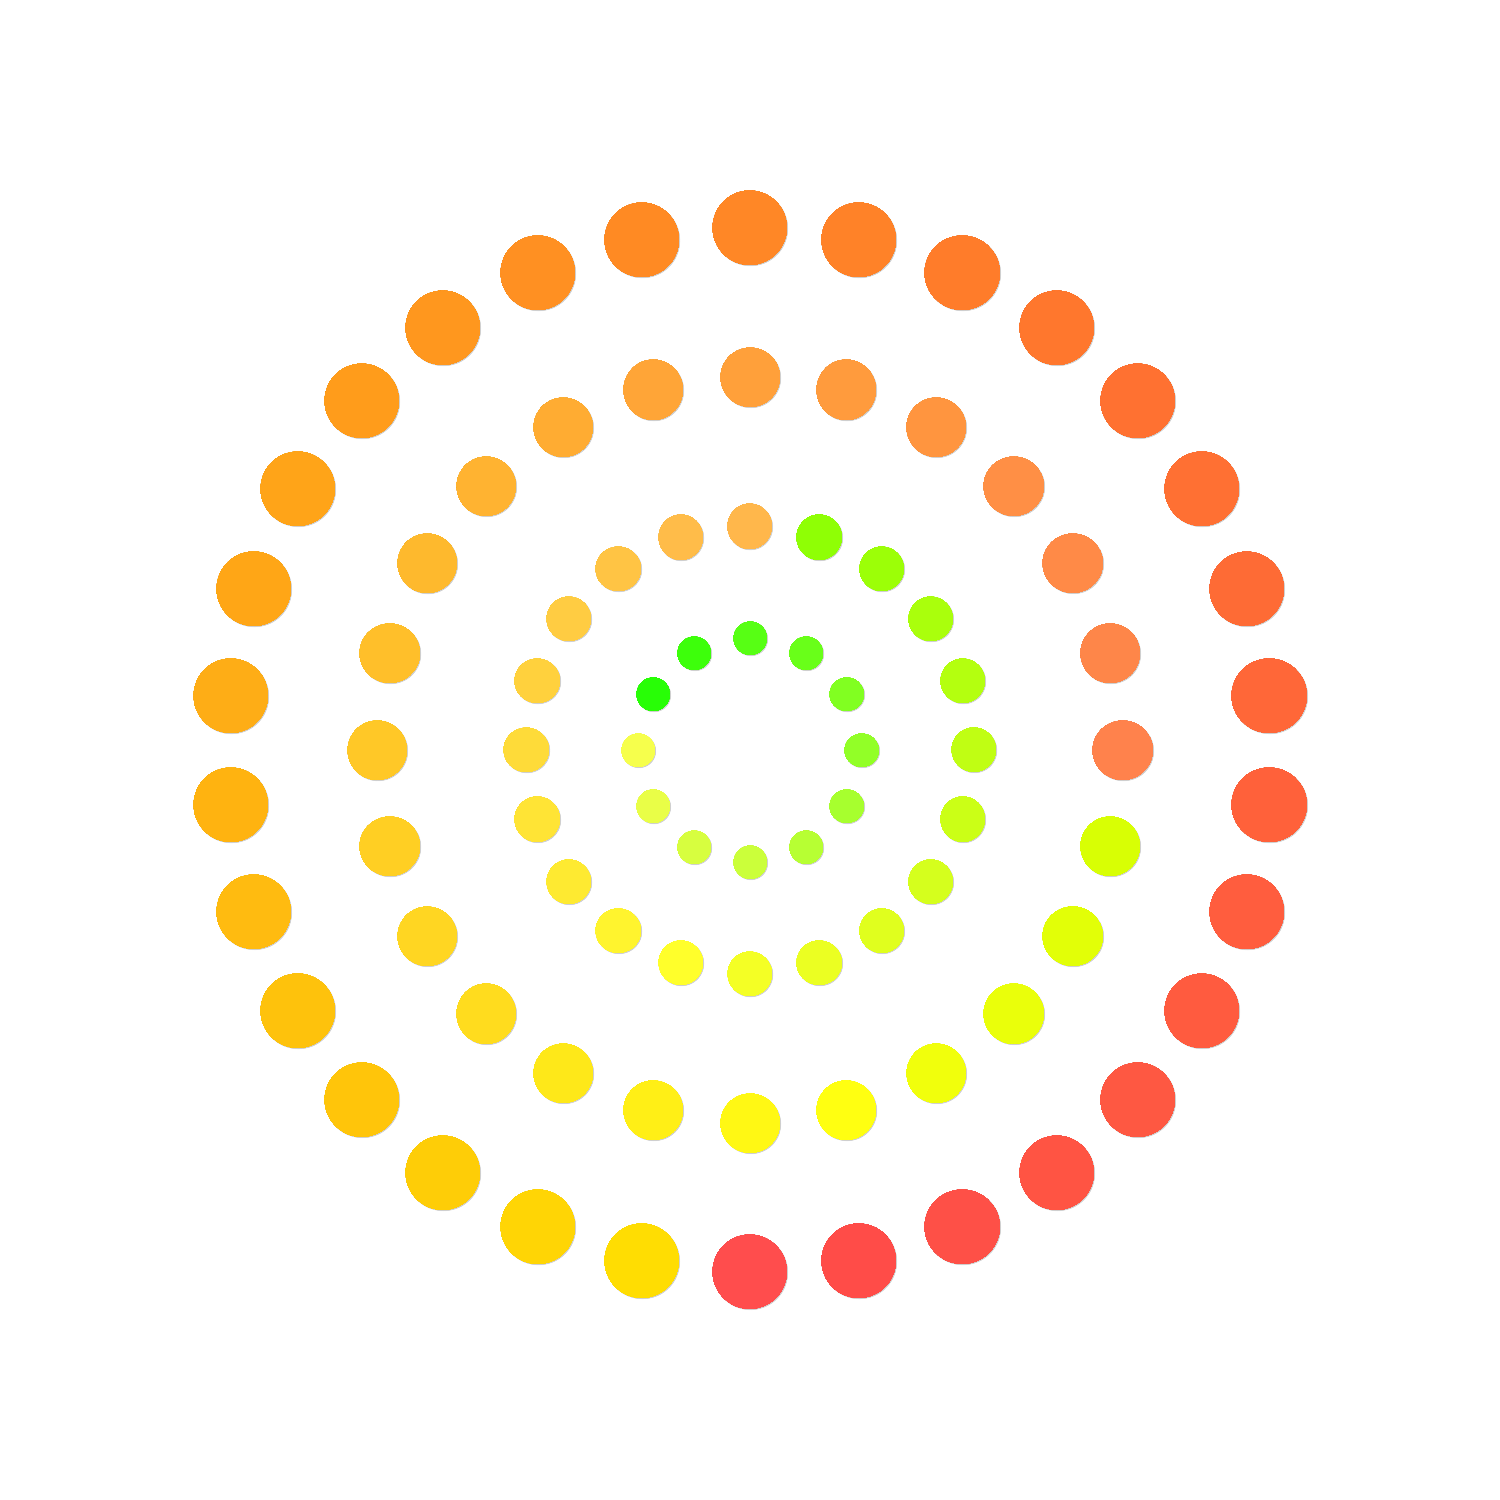
\includegraphics[width=0.9\columnwidth]{imgs/scene}}}
\caption{Une partition avec synchronisation imbriquée.}
\label{fig:scene}
\end{figure}



%=============================================================
\section{Conclusion}

La méthode proposée pour la synchronisation graphique d'objets arbitraires en fonction de leurs relations temporelles combine les avantages de la simplicité et de la flexibilité : une grande diversité de comportements peut être décrite par la simple définition de segmentations et de mappings. Cette méthode est décrite indépendamment de toute implémentation.

La simplicité et la flexibilité caractérisent également l'approche mise en oeuvre pour intégrer la représentation de l'interprétation au sein de la partition. Elle consiste à abstraire le calcul de la représentation du moteur de rendu, ce qui en fait un système ouvert et dynamiquement extensible.

Il y a de nombreux domaines d'application potentiels au concept de partition augmentée - domaine pédagogique, jeux,... - mais nous souhaitons également que ce travail puisse servir les besoins de la création contemporaine et notamment de ses nouvelles formes telles que les musiques interactives.


%=============================================================
\vspace{4mm}
\hspace{-5mm}
\textbf{Remerciements} \\
Cette recherche a été menée dans le cadre du projet Interlude qui est soutenu par l'Agence Nationale pour la Recherche [ANR-08-CORD-010].

%\bibliographystyle{unsrt}
\bibliographystyle{IEEEtranS}
\bibliography{../interlude}

\end{document}
